\documentclass[aspectratio=169]{beamer}

\mode<presentation>
{
  \usetheme{default}
  \usecolortheme{default}
  \usefonttheme{default}
  \setbeamertemplate{navigation symbols}{}
  \setbeamertemplate{caption}[numbered]
  \setbeamertemplate{footline}[frame number]  % or "page number"
  \setbeamercolor{frametitle}{fg=white}
  \setbeamercolor{footline}{fg=black}
} 

\usepackage[english]{babel}
\usepackage[utf8x]{inputenc}
\usepackage{tikz}
\usepackage{courier}
\usepackage{array}
\usepackage{bold-extra}
\usepackage{minted}
\usepackage[thicklines]{cancel}

\xdefinecolor{dianablue}{rgb}{0.18,0.24,0.31}
\xdefinecolor{darkblue}{rgb}{0.1,0.1,0.7}
\xdefinecolor{darkgreen}{rgb}{0,0.5,0}
\xdefinecolor{darkgrey}{rgb}{0.35,0.35,0.35}
\xdefinecolor{darkorange}{rgb}{0.8,0.5,0}
\xdefinecolor{darkred}{rgb}{0.7,0,0}
\definecolor{darkgreen}{rgb}{0,0.6,0}
\definecolor{mauve}{rgb}{0.58,0,0.82}

\title[2017-10-11-rootioworkshop-lz4-bulkio-nanoaod]{LZ4, BulkIO, and offset removal performance}
\author{Jim Pivarski}
\institute{Princeton University -- DIANA}
\date{October 11, 2017}

\begin{document}

\logo{\pgfputat{\pgfxy(0.11, 7.4)}{\pgfbox[right,base]{\tikz{\filldraw[fill=dianablue, draw=none] (0 cm, 0 cm) rectangle (50 cm, 1 cm);}
\includegraphics[height=1 cm]{diana-hep-logo.png}}}}

\begin{frame}
  \titlepage
\end{frame}

% Uncomment these lines for an automatically generated outline.
%\begin{frame}{Outline}
%  \tableofcontents
%\end{frame}

%%%%%%%%%%%%%%%%%%%%%%%%%%%%%%%%%%%%%%%%%%%%%%%%%%%%%%%

%%%% START

\begin{frame}{Motivation for this study}
\vspace{0.15 cm}
Three updates to ROOT I/O are aimed at speeding up or reducing file size for end-user analysis:
\begin{itemize}
\item new compression algorithm: LZ4 (speed)
\item reading TBasket data directly into arrays: BulkIO (speed)
\item removing offset data from TBranches that have a counter (size)
\end{itemize}

\vspace{0.5 cm}
\begin{uncoverenv}<2->
Focus on CMS NanoAOD in particular because
\begin{itemize}
\item it is aimed at end-users (1--2~kB/event)
\item it is broadly intended for 30--50\% of analyses (not an individual user's ntuple)
\end{itemize}
\end{uncoverenv}

\vspace{0.5 cm}
\begin{uncoverenv}<3->
Also including studies of LHCb (thanks, Oksana!).

\vspace{0.2 cm}
No ATLAS files because I can't generate new ones or {\tt TTree::CopyTree} old ones.
\end{uncoverenv}
\end{frame}

\begin{frame}{Parameters of the NanoAOD studies}
\vspace{0.25 cm}
\begin{center}
\begin{minipage}{0.9\linewidth}
\begin{itemize}
\item AWS instance with a fast SSD disk (i2.xlarge).
\item No resource contention because I paid for exclusive access.
\item ``Writing'' means a {\tt TTree::CopyTree} with new TFile compression.
\item ``Reading'' means filling a class made by MakeClass.
\item ``BulkIO'' means filling arrays through {\tt GetEntriesSerialized}.
\item Always {\it reading} from warmed cache.
\item Five repeated trials; standard deviations are small compared to trends.
\end{itemize}
\end{minipage}
\end{center}
\end{frame}

\begin{frame}{LZ4 doesn't compress as well as ZLIB, LZMA}
\vspace{0.1 cm}
\begin{center}
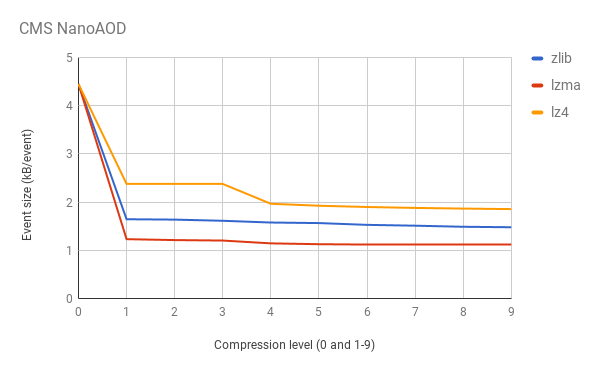
\includegraphics[width=0.9\linewidth]{size-vs-compression.png}
\end{center}
\end{frame}

\begin{frame}{But it's faster: level 1--3 are as fast as writing uncompressed}
\vspace{0.1 cm}
\begin{center}
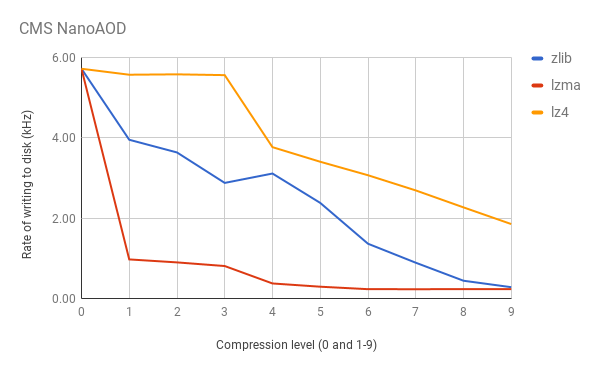
\includegraphics[width=0.9\linewidth]{write-vs-compression.png}
\end{center}
\end{frame}

\begin{frame}{More importantly: reading is as fast as uncompressed}
\vspace{0.1 cm}
\begin{center}
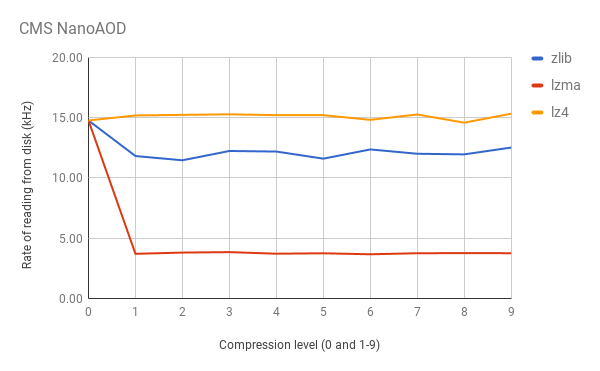
\includegraphics[width=0.9\linewidth]{read-vs-compression.png}
\end{center}
\end{frame}





\end{document}
